\section{Evaluation}

We implement a fragment of web layout in Megatron
  and use it to compare Spineless Traversal
  against Double Dirty Bit
  on \NumWebsites real-world websites.

\subsection{Web Layout Fragment}
\label{sec:layout-impl}

Existing web layout implementations
  are complex and tightly coupled
  to their current invalidation strategy.
Therefore, to evaluate Spineless Traversal,
  we re-implemented web layout, 
  basing our approach on Cassius and \textsc{Medea}%
  ~\cite{cassius-1,cassius-2,yufeng-2}.
Naturally, our implementation handles only a subset
  of HTML and CSS features.
However, we took care to implement several features
  with complex invalidation behavior described below.
In total, our implementation computes approximately 50 layout fields
  over about 700 lines of Megatron DSL.

\paragraph{Box model}
Each layout node has $x$, $y$, \textsf{width} and \textsf{height} fields;
  formally, this rectangle defines its border box.
Typically a node's border box contains its children
  and doesn't overlap with siblings.
Width generally has parent-to-child dependencies,
  height generally has child-to-parent dependencies,
  while $x$ and $y$ are computed in-order.
This forms long dependency chains between elements---%
  modifying one element can eventually dirty many others---%
  but many CSS properties like
  \textsf{width}, \textsf{min-width}, and \textsf{max-width},
  and similar for \textsf{height},
  can break these dependency chains.
These properties, however, allow values like \textsf{50\%},
  which are resolved relative to the parent and thus
  still creates inter-node dependencies.
	
\paragraph{Line Breaking}
Line breaking lays out inline layout nodes (text)
  horizontally into lines.
When text reaches the right edge of its parent box,
  the next inline layout node is placed in the next line.
Line breaking thus creates control dependencies,
  where checking the parent node's width may cause layout nodes
  to move from one line to another (by changing line breaking).
Additionally, our layout algorithm
  allows different lines to have different heights
  (based on the height of the largest layout node in the line),
  which introduces a field (line height)
  that is dependent on many different nodes (each word in the line).
This also requires multiple layout passes,
  since later words in a line
  can affect the placement of earlier words
  by adjusting the text baseline.
This has a number of interesting effects for invalidation.
For example, adding a node to a line
  may or may not change the line's height,
  depending on whether the new node is tallest.
If it is, all other text on the page must move down,
  causing a lot of invalidation.

\paragraph{Display}
The \textsf{display} property changes
  whether a node acts like words (\textsf{inline})
  or paragraphs (\textsf{block}).
It can also be \textsf{none},
  in which case the layout nodes are not shown on the page
  and have almost no effect on layout;
  changing \textsf{display} between \textsf{block} and \textsf{none}
  is a common way to implement drop-down menus, pop-ups, and tool-tips.
Importantly, \texttt{<script>} and \texttt{<style>} tags
  have \textsf{display: none};
  inserting them into the page must be fast.

\paragraph{Position}
An element with \textsf{position: absolute}
  is manually assigned its $x$ and $y$ position by the web developer;
  this property is used for popups, tool-tips, and other hover effects.
It is also common
  to change the manually-assigned $x$ and $y$ positions
  from JavaScript, such as to move a tool-tip away from the cursor.
Layout nodes with absolute positioning do not affect
  the position of sibling layout nodes,
  and handling changes to $x$ and $y$ positions quickly is essential.

\paragraph{Intrinsic sizes}
Layout nodes have an ``intrinsic'' size---%
  its size without any or with all line breaks, basically---%
  which is used for, for example, absolutely-positioned elements.
Importantly, intrinsic widths are computed bottom-up,
  but are then used in the top-down width computation,
  which then affects the bottom-up height computation.
This means intrinsic sizes require the use of
  multiple layout phases.

\paragraph{Flexbox}
Flexbox layout is the most complex feature we implemented.
In flexbox layout there is flex container element
  whose children are flex items.
The width/height of flex items depends on
  the intrinsic sizes of the other flex items and
  the actual size of the flex container.
Properties like \textsf{flex-grow} and \textsf{flex-shrink}
  determine how the intrinsic sizes of the flex items
  are adjusted to match available space in the flex container.
The \textsf{max-} and \textsf{min-width}/\textsf{height} properties
  can also cap the growth/shrinkage of individual flex items.
In all, our implementation of flexbox layout
  uses 9 intermediate fields
  and requires 2 passes to compute all of them.
Note that the full web layout specification
  includes layout modes like grid layout,
  which require even more passes.

\paragraph{Miscellaneous}
We also implemented a variety of miscellaneous features,
  including automatic sizing of images and video,
  manual line breaks with the \texttt{<br>} element,
  and hidden elements like \texttt{<noscript>}
  (which are only rendered if JavaScript is disabled).
We also had to add a special case for \texttt{<svg>} elements,
  whose children describe drawing commands
  that do not participate in layout.
Finally, we also implemented the \textsf{width} and \textsf{height}
  HTML attributes
  (which behave slightly differently from the CSS properties).

\subsection{Benchmark Web Pages}

To capture web layout traces,
  we modified the Ladybird web browser
  to dump the layout tree at every rendered frame,
  including attributes and properties for each node;
  we then use a separate program to ``diff'' successive frames,
  outputting a list of insertions, deletions,
  and attribute/property changes for that frame.
The driver program then reads each frame from the trace,
  performs each modification in the frame,
  and finally invokes incremental layout for that frame.
In total, we captured traces from \NumWebsites websites,
  and those traces contain  \NumFrames frames in total;
  in our evaluation, each frame is one data point.
Note that this large number of frames,
  covering gigabytes of layout tree data,
  nonetheless represents only a few minutes of web browsing activity.
All experiments are run on a machine with
  an Intel i7-8700K CPU (8th generation)
  clocked at the standard 3.70\,GHz
  with 64\,KB L1 cache, 256\,KB L2 cache (both per core),
  and 12\,MB L3 cache (shared), plus
  32\,GB of DDR4 memory across 4 DIMMs at 3000 MT/s.

The \NumWebsites real-world websites include
  Amazon, Wikipedia, Github, Google,
  as well as a number of other
  large web pages and complex web applications
  drawn from the Alexa ranking of top websites.
A number of the authors' personal favorites are also included,
  such as Github and Lichess.

We focus on latency-sensitive interactions
  like hovering, typing, dragging, and animations.
These interactions typically
  do not require loading data over the network
  and invalidation time is thus a big determinant of their latency.
Even though the interactions may seem minor,
  it is important to note that the browser is nonetheless
  performing a significant amount of work to render them.
For example, on Wikipedia, hovering over a link
  fades a ``preview'' window in and out,
  and Wikipedia code must track and respond to mouse movements
  to hide and show the preview window at the correct time.
Moreover, there is a short, nearly-imperceptible animation
  by which the preview window slides and fades in and out of view.
Similarly, on the Lichess web page,
  our trace captures one of the authors
  stepping through a chess opening using the website's
  chess commentary tools.
The Lichess website renders the chess board using HTML elements
  and each move animates visual aids like arrows.
Text editing, an especially latency-sensitive interaction,
  was also tested.
For example, on the Google website we tested
  typing a search term letter by letter,
  with the Google website changing autocomplete suggestions
  as we typed.
Executing these interactions at low latency
  is critical for avoiding ``jank''.

\subsection{Results}

\begin{figure}
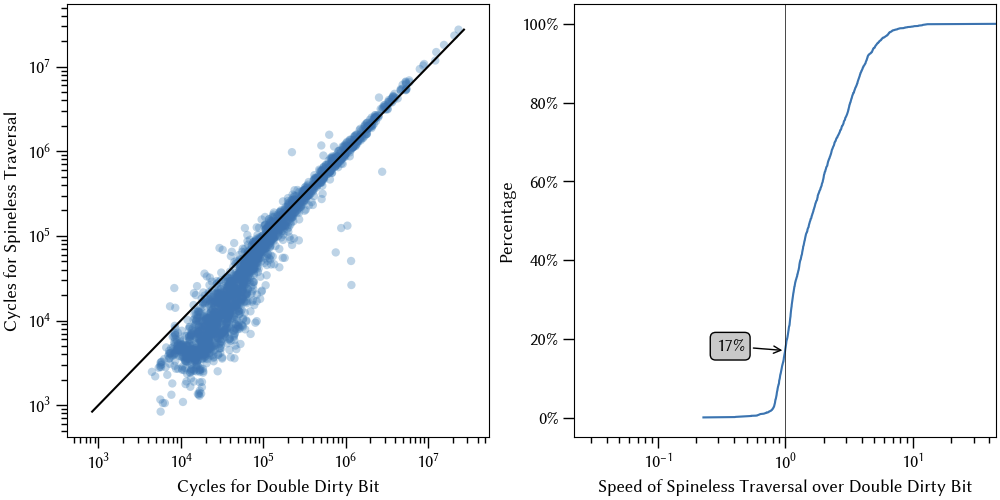
\includegraphics[scale=0.4]{DBPQ.png}
\begin{minipage}[t]{0.48\linewidth}
\caption{
Re-layout time for all \NumFrames frames,
    with Double Dirty Bit time on the $x$ axis
    and Spineless Traversal time on $y$ axis.
The diagonal $x = y$ line shows equal time;
    points below the line are faster with Spineless Traversal
    while points above the line are faster with Double Dirty Bit.
Both axes are in log scale, meaning Spineless Traversal is often
    many faster than Double Dirty Bit.
}
\label{fig:xy}
\end{minipage}\hfill%
\begin{minipage}[t]{0.48\linewidth}
\caption{
  A CDF of the ratio between
    Double Dirty Bit time and Spineless Traversal time
    for each frame.
  The vertical line, at $10^0 = 1\times$,
    marks where both invalidation algorithms take equal time.
  To the left of the line,
    \PctSlower of frames are slower with Spineless Traversal.
  To the right of the line,
    \PctFaster of frames are faster with Spineless Traversal.
  The geometric mean speedup with Spineless Traversal
    is \MeanSpeedup.}
\label{fig:cdf}
\end{minipage}
\end{figure}

\iffalse
\begin{figure}
\begin{subfigure}{0.5\linewidth}
    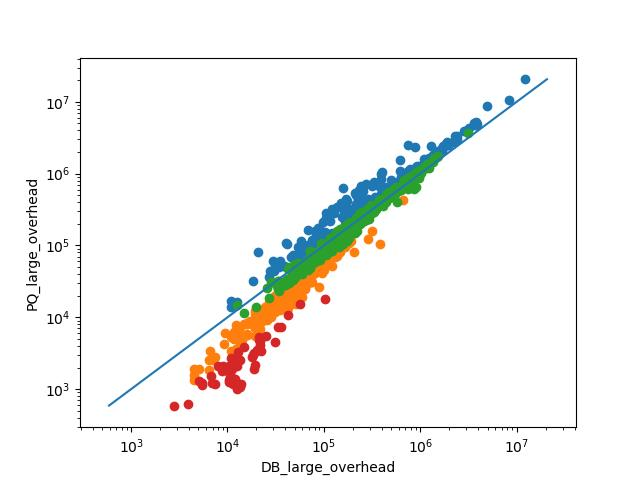
\includegraphics[width=\linewidth]{DBPQLargeOverhead.png}
\end{subfigure}\hfill%
\begin{subfigure}{0.5\linewidth}
    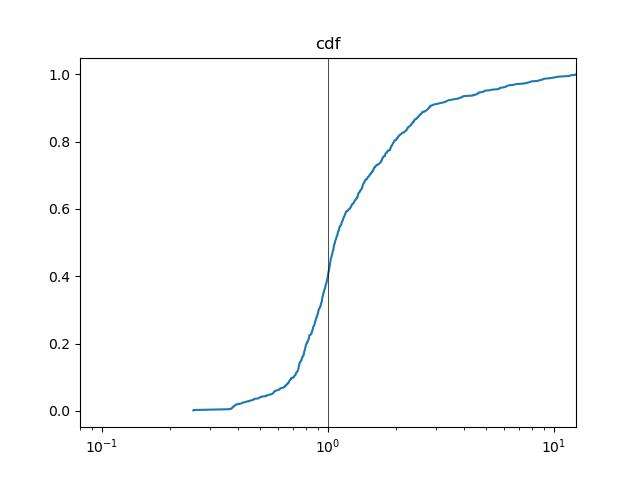
\includegraphics[width=\linewidth]{DBPQLargeCDF.png}
\end{subfigure}
\caption{
The overhead scatter plot and the speedup cdf,
  restricted to frames where more than 1\% of fields
  are recomputed. These points typically represent loading of new contents.}
\label{fig:dbpq-large}
\end{figure}
\fi

\Cref{fig:xy}
  shows our results.
In it, points below the diagonal line
  are frames that are faster with Spineless Traversal,
  while points above the diagonal line
  are frames faster with Double Dirty Bit.
Most frames are below the line:
  only a few deeply-nested nodes are dirtied,
  but Double Dirty Bit makes a huge number of auxiliary accesses,
  which Spineless Traversal avoids.
By contrast, while some points are above the line,
  meaning they are slower with Spineless Traversal,
  the slowdowns are typically much less severe.
The geometric mean is a \MeanSpeedup speedup
  from Spineless Traversal,
  with only \PctSlower of frames rendered slower,
  as shown in \Cref{fig:cdf}.
\Cref{fig:nodes-accessed} shows the reason for this speedup:
  Spineless Traversal simply accesses far fewer nodes
  than Double Dirty Bit.

\Cref{fig:xy,fig:cdf} includes both
  ``overhead'' and ``evaluation'' time.
Evaluation time, as expected, is nearly identical
  between Spinless Traversal and Double Dirty Bit.
Considering overhead alone,
  Spineless Traversal is, for some frames,
  as much as $100\times$ faster than Double Dirty Bit.
For Spineless Traversal,
  overhead time was roughly one third of total runtime,
  while evaluation time was roughly two thirds,
  showing that invalidation overhead is still
  a significant determinant of latency.
Naturally, the slower Double Dirty Bit algorithm
  spends even more time in invalidation overhead.
Breaking overhead time down further for Spineless Traversal
  shows that both the priority queue
  and the order maintenance structure
  contribute to overhead, with different algorithms
  dominating for different benchmarks

A careful inspection of \Cref{fig:xy} shows
  several additional features.
The slowest frames all feature slowdowns.
This is expected: the slowest frames likely represent
  the initial page load or other ``loading'' frames,
  which we necessarily capture in our traces.
While speedups are always better than slow-downs,
  these loading frames likely follow network latency,
  so invalidation time for these frames is less important.
Meanwhile, frames where fewer nodes are invalidated
  are typically those triggered in response to
  an animation or user interaction,
  where latency is most noticeable as ``jank''.
When we restrict the data to only include frames
  where fewer than 1\% of fields are recomputed---%
  the intention being to ignore ``loading'' frames---%
  the geometric mean speedup is larger,
  at \MeanSpeedupSmall,
  and a smaller fraction of frames (\PctSlowerSmall) suffer slowdowns.
Spineless Traversal is also faster outside this subset,
  likely because the 1\% threshold is an imprecise heuristic,
  but the larger speedup 
  in this latency-critical subset is indicative.

\begin{figure}
\begin{minipage}{.59\linewidth}%
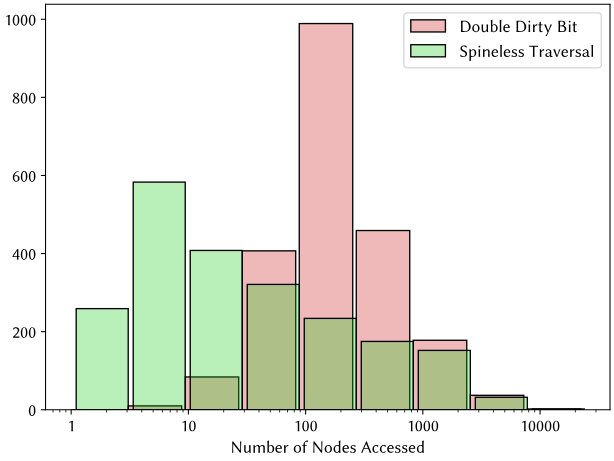
\includegraphics[width=\linewidth]{DBPQHist.png}%
\caption{Histograms of Number of Nodes Accessed by Double Dirty Bit and Spineless Traversal. Double Dirty Bit access much more nodes compare to Spineless Traversal, so the latter cause much fewer cache misses.}
\label{fig:nodes-accessed}
\end{minipage}\hfill%
\begin{minipage}{.39\linewidth}%
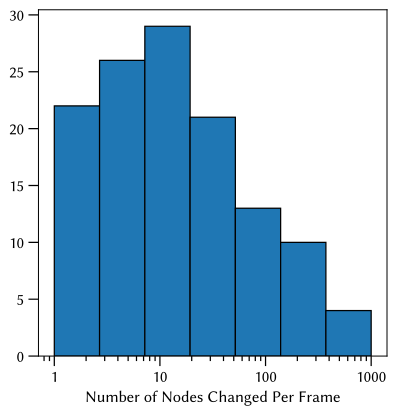
\includegraphics[width=\linewidth]{CaseStudy.png}
\caption{The numbers of Twitter nodes changed externally for each frame. Most frames modify very few nodes, but a few frames insert/remove large subtrees of up to 787 nodes.}
\label{fig:case-study}
\end{minipage}
\end{figure}

\subsection{Case Study: Twitter}

We now focus specifically
  on our trace of Twitter (now X), a social media platform.
This trace of 125 frames captures the user
  opening the Twitter news feed,
  loading the default number of tweets,
  and scrolling down repeatedly to load more tweets.
Twitter is a large web page,
  and the tree grows to 3\thinspace700 DOM nodes
  with a depth of 53 and a fanout of 128. 
Considering all the frames in aggregate,
  Twitter sees a geometric mean speedup of $1.99\times$ 
  over the Double Dirty Bit algorithm.

Most of the 125 incremental layouts are small,
  dirtying no more than 20 nodes (Figure~\ref{fig:case-study}).
For these frames,
  Double Dirty Bit spends most of its time
  accessing auxiliary nodes.
However, the largest incremental layout
  dirties several hundred nodes.
We now discuss several common kinds of frames
  in the Twitter trace.

\paragraph{Linked Files}
Many layouts are triggered when linked files---%
  JavaScript, CSS, images, and videos---%
  finish loading.
Loading JavaScript might add
  new \texttt{<script>} and \texttt{<style>} elements to the page,
  while loading CSS files can change the CSS properties
  of existing elements.
Loading images and videos, meanwhile,
  changes intrinsic widths and heights
  from 0 to the actual image/video width/height.
Typically only one or a few nodes are dirtied,
  but these nodes are often located deep in the layout tree
  or have many siblings,
  so they have many auxiliary nodes.
Spineless Traversal thus reduces latency for these frames
  by up to $10\times$.
 
\paragraph{Lazy Loading}
Twitter uses a lazy-loading technique
  which first loads a ``shell'' page
  and then gradually adds more and more elements to the shell
  as more content is loaded over the network.
For example, the header bar, side bar, ads, and tweets
  all load separately and require separate incremental layouts.
Scrolling causes yet more content (tweets and ads) to load.
Each of these frames typically involve inserting
  a single large subtree.
Allocating the new nodes' OM objects
  (and possibly rebalancing the OM data structure)
  makes these frames difficult for Spineless Traversal
  despite its bulk insertion optimizations,
  Spineless Traversal is slower than Double Dirty Bit,
  typically by about $2\times$.
That said, the latency
  is partially hidden by the network latency
  of loading the content in the first place,
  so the slowdown here may be less critical
  than for other frames.

\paragraph{Removal}
The Twitter application also occasionally removes
  subtrees that are no longer visible to the user,
  like offscreen content.
Spineless Traversal handles these removals
  much faster than Double Dirty Bit,
  often by $5\times$ or more,
  precisely because these removals
  do not affect what the user sees on the screen.
Twitter also sometimes removes
  individual \texttt{<script>} and \texttt{<style>} elements
  that don't affect the page;
  here Spineless Traversal's speedup
  is smaller, approximately $2\times$,
  as multiple elements are removed at once,
  amortizing the auxiliary accesses in Double Dirty Bit. 

Moreover,
  some frames mix file loading, lazy loading, and removals,
  probably at the whim of the task scheduler.
Often many images load in at once.
In this case the time taken for Spineless Traversal 
  basically sums over the time for each individual change,
  while Double Dirty Bit can amortize the cost
  of traversing auxiliary nodes.
These frames are often small,
  so Spineless Traversal's speed-ups are still substantial,
  but probably smaller than if each modification
  was laid out in its own frame.
